\iffalse
\def\mytitle{PARALLELOGRAM}
\def\myauthor{VUNNAVA SRAVANI}
\def\contact{sravani21vunnava@gmail.com}
\def\mymodule{Future Wireless Communication (FWC)}
\documentclass[10pt, a4paper]{article}
\usepackage[a4paper,outer=1.5cm,inner=1.5cm,top=1.75cm,bottom=1.5cm]{geometry}
\twocolumn
\usepackage{setspace}
\doublespacing
\usepackage{graphicx}
\graphicspath{{./images/}}
\usepackage[colorlinks,linkcolor={black},citecolor={blue!80!black},urlcolor={blue!80!black}]{hyperref}
\usepackage[parfill]{parskip}
\usepackage{lmodern}
\usepackage{tikz}
	\usepackage{physics}
%\documentclass[tikz, border=2mm]{standalone}
\usepackage{karnaugh-map}
%\documentclass{article}
\usepackage{tabularx}
\usepackage{circuitikz}
\usetikzlibrary{calc}
\usepackage{amsmath}
\usepackage{amssymb}
\renewcommand*\familydefault{\sfdefault}
\usepackage{watermark}
\usepackage{lipsum}
\usepackage{xcolor}
\usepackage{listings}
\usepackage{float}
\usepackage{titlesec}
\providecommand{\mtx}[1]{\mathbf{#1}}
\titlespacing{\subsection}{1pt}{\parskip}{3pt}
\titlespacing{\subsubsection}{0pt}{\parskip}{-\parskip}
\titlespacing{\paragraph}{0pt}{\parskip}{\parskip}
\newcommand{\figuremacro}[5]{
    \begin{figure}[#1]
        \centering
        \includegraphics[width=#5\columnwidth]{#2}
        \caption[#3]{\textbf{#3}#4}
        \label{fig:#2}
    \end{figure}
}
\newcommand{\myvec}[1]{\ensuremath{\begin{pmatrix}#1\end{pmatrix}}}
\let\vec\mathbf
\lstset{
frame=single, 
breaklines=true,
columns=fullflexible
}

%\thiswatermark{\centering \put(181,-119.0){\includegraphics[scale=0.13]{IIT_logo.png}} }
\title{\mytitle}
\author{\myauthor\hspace{1em}\\\contact\\FWC22012\hspace{6.5em}IITH\hspace{0.5em}\mymodule\hspace{6em}ASSIGN-5}
\date{}
\begin{document}
	\maketitle
	\tableofcontents
   \section{Problem}
   \fi
  $ABCD$ is a parallelogram and $AP$ and $CQ$ are
perpendiculars from vertices $\vec{A}$ and $\vec{C}$ on diagonal
$BD$ . Show that 
\begin{enumerate}
	\item  $\triangle APB \cong \triangle CQD$   
		\label{prob:9/8/1/10/1}
	\item  $AP = CQ$
		\label{prob:9/8/1/10/2}
\end{enumerate}

 	\begin{figure}
		\centering
 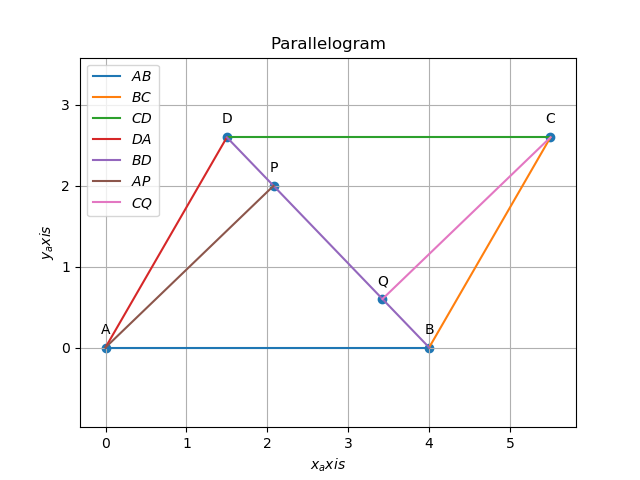
\includegraphics[width=\columnwidth]{chapters/9/8/1/10/figs/matrix_line.png}
		\caption{}
		\label{fig:9/8/1/10}
  	\end{figure}
\solution From Fig. 
		\ref{fig:9/8/1/10},
		and 
    \eqref{eq:angle2d},
\begin{align}
		\begin{split}
	\cos \angle{ABD}
	&= \frac{(\vec{A}-\vec{B})^T(\vec{D}-\vec{B})}{\norm{\vec{A}-\vec{B}}\norm{\vec{D}-\vec{B}}}
	\\
\cos	\angle{CDB}
	 &= \frac{(\vec{C}-\vec{D})^T(\vec{B}-\vec{D})}{\norm{\vec{C}-\vec{D}}\norm{\vec{B}-\vec{D}}}
		\end{split}
	 \label{eq:9/8/1/10/cang}
%
\end{align}
From Appendix 
	  \ref{eq:two-pgm}, 
\begin{align}
\vec{A}
-
\vec{B}
=
	\vec{D}
-\vec{C}
\end{align}
Substituting in 
	 \eqref{eq:9/8/1/10/cang},
\begin{align}
	\cos \angle{ABD}
	=\cos \angle{CDB}
\end{align}
Using SAS congruence, 
		\ref{prob:9/8/1/10/1}  is proved. \ref{prob:9/8/1/10/2} follows from 
\ref{prob:9/8/1/10/1}.
\iffalse

	   % 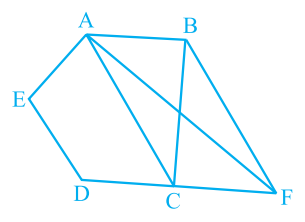
\includegraphics[scale=1.0]{diag_1.png}
   \section{Solution}

The input parameters for this construction are 
\begin{center}
\begin{tabular}{|c|c|}
	\hline
	\textbf{Symbol}&\textbf{Value}\\
	\hline
	b&6\\
	\hline
	r&5\\
	\hline
	$\theta$&$\frac{\pi}{3}$\\
	\hline
\end{tabular}
\begin{center}
$\vec{A}=\myvec{0\\0}$\\
$\vec{D}=\myvec{r\cos\theta \\ r\sin\theta}$\\
$\vec{B}=\myvec{0\\b}$\\
$\vec{C} = \vec{B}+\vec{C}$
\end{center}
\end{center}
\textbf{To Prove:} AP = CQ
\fi
\iffalse
		\begin{center}
		The line equation for diagonal BD is $x = \vec{B}+\lambda\vec{m}$
		\\
		where $\vec{m} = \vec{B}-\vec{D}$\\
		
		then,\\
		
		$\vec{P} = \vec{B} - \frac{\vec{m}^T \vec{B}}{\norm{\vec{m}}^2}\vec{m}$
	\\
	
	$\vec{Q} = \vec{B} - \frac{\vec{m}^T \vec{B-C}}{\norm{\vec{m}}^2}\vec{m}$\\
	\end{center}
	
	distance between A and P is $\norm{\vec{A-P}}$\\
	distance between C and Q is $\norm{\vec{C-Q}}$\\
	if $\norm{\vec{A-P}}$ =  \\
	then AP = CQ..........(1)
	
	\textbf{To Prove:}  $\triangle APB \cong \triangle$ CQD\\
	to prove $\angle {APD}=\angle {CQD}=90^{\circ}$\\
	$\vec{m1} = \vec{A-P}$\\
	$\vec{m2} = \vec{P-B}$\\
	$\theta= \angle {APD}$ \\
	 $\cos\theta$ = $\frac{\vec{m1}^T \vec{m2}}{\norm{\vec{m1}}\norm{\vec{m2}}}$\\
	$\theta = 90^{\circ}, cos\theta$ = 0\\
	$\therefore m1^T m2 = 0$\\
	$\vec{n1} = \vec{C-Q}$\\
	$\vec{n2} = \vec{Q-D}$\\
	$\theta = \angle{CQD}$\\
	$cos\theta$ = $\frac{\vec{n1}^T \vec{n2}}{\norm{\vec{n1}}\norm{\vec{n2}}}$\\
	f $\theta$ = 90$^{\circ}, cos\theta$ = 0\\
	$\therefore n1^T n2 = 0$\\
	\begin{center}
	if 	$m1^T m2 = n1^T n2$ = 0\\
	then, $\angle {APD} = \angle {CQD} = 90^{\circ}$..........(2)\\
	\end{center}
	to prove $\angle {ABP}=\angle {CDQ}$ \\
	$\vec{m2} = \vec{P-B}$\\
	$\vec{m3} = \vec{A-B}$\\
	$\theta1 = \angle {ABP}$\\
	$\theta1 = \cos^-1\frac{\vec{m2} \cdot \vec{m3}}{\norm{\vec{m2}}\norm{\vec{m3}}}$\\
	$\vec{n2} = \vec{C-D}$\\
	$\vec{n3} = \vec{Q-D}$\\
	$\theta2 = \angle {CDQ}$\\
	$\theta2 = \cos^-1\frac{\vec{n2} \cdot \vec{n3}}{\norm{\vec{n2}}\norm{\vec{n3}}}$\\
	\begin{center}
	 		if $\theta1 = \theta2$\\
	 		then $\angle {ABP} = \angle {CQD}$..........(3)
	\end{center}
	\begin{center}
$\therefore$ from (1),(2) and (3)
$\triangle APB \cong \triangle CQD$ 
	\end{center}
\begin{lstlisting}
https://github.com/sravani21vunnava/sravani21vunnava/blob/main/Matrices_line/codes/matrix_line.py
\end{lstlisting}
 
\section{Construction}
 	
\bibliographystyle{ieeetr}
\end{document}
\fi
